\documentclass[conference]{IEEEtran}
\IEEEoverridecommandlockouts

\usepackage{iftex}
% IEEEtran selects Times under pdfLaTeX; XeTeX/LuaTeX need it set explicitly.
\ifPDFTeX\else
  \usepackage{fontspec}
  \setmainfont{texgyretermes}[Extension=.otf, UprightFont=*-regular, BoldFont=*-bold,
    ItalicFont=*-italic, BoldItalicFont=*-bolditalic]
\fi
\usepackage{cite}
\usepackage{amsmath,amssymb,amsfonts}
\usepackage{graphicx}
\usepackage{textcomp}
\usepackage{xcolor}
\usepackage{url}
\usepackage{booktabs}
\usepackage{balance}

\graphicspath{{figures/}}

\begin{document}

\title{Secure Audit:\\
Digital Evidence and Investigation Support System}

\author{
\IEEEauthorblockN{Ancilla Teresa Dsouza}
\IEEEauthorblockA{\textit{Computer Science and Engineering}\\
\textit{St Joseph Engineering College}\\
Mangaluru, India\\
23a22.ancilla@sjec.ac.in}
\and
\IEEEauthorblockN{Amisha Josna Dsouza}
\IEEEauthorblockA{\textit{Computer Science and Engineering}\\
\textit{St Joseph Engineering College}\\
Mangaluru, India\\
23a17.amisha@sjec.ac.in}
\and
\IEEEauthorblockN{Alisha Anton Fernandis}
\IEEEauthorblockA{\textit{Computer Science and Engineering}\\
\textit{St Joseph Engineering College}\\
Mangaluru, India\\
23a14.alisha@sjec.ac.in}
\and
\IEEEauthorblockN{Apeksha A Govekar}
\IEEEauthorblockA{\textit{Computer Science and Engineering}\\
\textit{St Joseph Engineering College}\\
Mangaluru, India\\
23d49.apeksha@sjec.ac.in}
\and
\IEEEauthorblockN{Shivangi M\textsuperscript{*}}
\IEEEauthorblockA{\textit{Computer Science and Engineering}\\
\textit{St Joseph Engineering College}\\
Mangaluru, India\\
shivangim@sjec.ac.in}
}

\maketitle

\begin{abstract}
Criminal investigations in India depend on evidence in many forms: First Information Reports (FIRs) written in several scripts, call recordings, crime-scene photographs and walkthrough videos. Each is usually examined with a separate tool, so an investigator cannot easily show that the file analysed is the file that was collected. This paper presents Secure Audit, an investigation support system that places five forensic analysis services behind one hash-verified evidence workflow. Every upload is fingerprinted with SHA-256 and anchored in an Ethereum smart contract before its database record is committed. Verification compares the stored file, the database copy and the on-chain digest, so file tampering, deletion and database manipulation are reported as distinct outcomes. The analysis layer provides line-level hybrid OCR for multilingual FIRs, a retrieval-augmented graph attention network for multi-label Bharatiya Nyaya Sanhita (BNS) section classification, electric network frequency (ENF) and spectral audio forensics, YOLOv8 weapon and person detection, and video-based 3D crime-scene reconstruction. Hybrid OCR reduced the mean character error rate from 4.45\% to 1.18\%. The integrity layer handled all 17 controlled tampering checks correctly at 509,737 gas per registration. The deployed BNS scorer recovered 91.5\% of manually assigned sections across 30 multi-offence FIRs, and video reconstruction reached an observation-weighted reprojection error of 0.876~px. The audio study also shows that low-pitched speech can imitate ENF anomalies, and that requiring agreement between independent indicators keeps these from becoming false tampering verdicts.
\end{abstract}

\begin{IEEEkeywords}
Digital forensics, chain of custody, blockchain, multilingual OCR, Bharatiya Nyaya Sanhita, graph attention networks, electric network frequency, YOLOv8, photogrammetry.
\end{IEEEkeywords}

%======================================================================
\section{Introduction}
%======================================================================

A single criminal case today can involve a photographed FIR that mixes English with Hindi or Kannada, a phone recording of a threat, surveillance stills, and a shaky walkthrough video of the scene. Each needs a different kind of analysis, usually in a different tool, and the weak point lies between the tools: a file that is copied, re-saved or quietly replaced leaves no reliable trace. In court, the investigator must show not only what the analysis found, but that it was performed on the original evidence.

Each of these problems has been studied on its own: blockchain custody ledgers~\cite{bonomi2018bcoc,li2021lechain}, photogrammetric scene reconstruction~\cite{sazaly3d,balbudhe2024}, knowledge-graph and retrieval models for crime and BNS analysis~\cite{kuok2024,mathias2024,dhanushkumar2024}, weapon detection~\cite{quyyum2024,werukanjana2024}, ENF audio forensics~\cite{ngharamike2023,pedapudi2024} and document OCR~\cite{alsayem2024}. What is missing is a workflow that ties these analyses to a verifiable record of the evidence they consumed.

Secure Audit fills this gap. Every file is hashed and anchored on an Ethereum smart contract before its database record exists, so verification can tell apart a modified file, a missing file, an unregistered file and a manipulated database row. Our contributions are:
\begin{enumerate}
    \item a hash-anchored evidence workflow whose dual-state check separates file tampering from database tampering;
    \item hybrid OCR that arbitrates between engines line by line for multilingual and mixed-script FIRs;
    \item a retrieval-augmented graph attention model, with an explainable deployed scorer, for multi-label BNS classification;
    \item audio tamper analysis that fuses ENF tracking with spectral indicators and requires agreement before a verdict;
    \item integrated weapon and person detection, and 3D scene reconstruction from ordinary walkthrough video.
\end{enumerate}

%======================================================================
\section{Related Work}
\label{sec:related}
%======================================================================

\textit{Evidence and custody.} Pedapudi and Vadlamani~\cite{pedapudi2024} describe the acquisition, hashing and analysis of audio and video evidence, and Kuok \textit{et al.}~\cite{kuok2024} answer investigative queries over a crime knowledge graph. B-CoC~\cite{bonomi2018bcoc} and LEChain~\cite{li2021lechain} record custody events on a blockchain, but neither links the ledger to later analysis; Secure Audit makes ledger verification the entry point to that analysis.

\textit{Forensic analysis.} Sazaly \textit{et al.}~\cite{sazaly3d} reconstruct indoor scenes with micro-UAV photogrammetry, and Balbudhe \textit{et al.}~\cite{balbudhe2024} review reconstruction techniques; we target the common case where only a handheld video exists. Al~Sayem \textit{et al.}~\cite{alsayem2024} show that Tesseract extraction depends strongly on image quality. Mathias \textit{et al.}~\cite{mathias2024} classify BNS sections with graph-based retrieval, and Dhanushkumar \textit{et al.}~\cite{dhanushkumar2024} survey NLP and generative AI for BNS guidance. Ngharamike \textit{et al.}~\cite{ngharamike2023} survey ENF-based multimedia forensics, while Quyyum and Abdullah~\cite{quyyum2024} and Werukanjana and Permpool~\cite{werukanjana2024} apply object detection to surveillance and crime-scene imagery.

%======================================================================
\section{System Architecture and Threat Model}
\label{sec:arch}
%======================================================================

\begin{figure*}[!t]
\centering
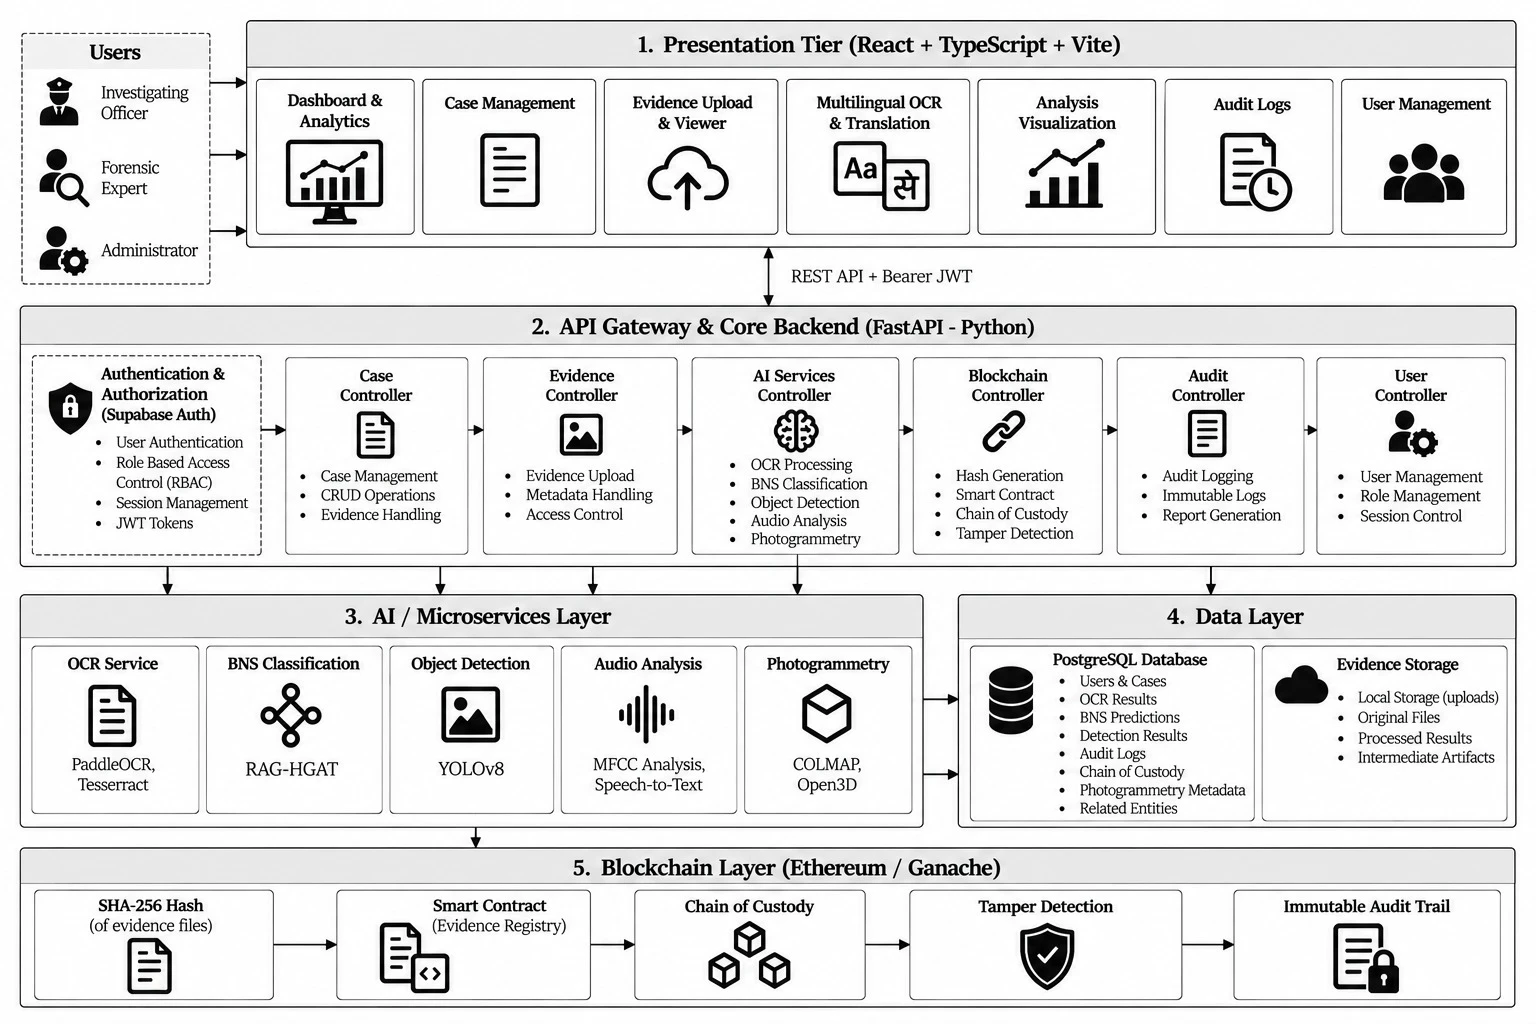
\includegraphics[width=0.78\textwidth]{fig_architecture.png}
\caption{Secure Audit architecture. A React client calls a FastAPI gateway over REST with bearer JWTs. The gateway enforces role-based access, routes work to five AI services, persists results in PostgreSQL, and anchors evidence digests in an Ethereum smart contract.}
\label{fig:architecture}
\end{figure*}

Secure Audit has five tiers (Fig.~\ref{fig:architecture}). The \textit{presentation tier} is a React~18/TypeScript application with case management, evidence upload, OCR and translation views, dashboards, audit logs and a Three.js scene viewer. The \textit{gateway} is a FastAPI service that authenticates users with bcrypt-hashed passwords, one-time e-mail codes and signed JWTs; administrators have global access, while investigators reach only their own cases. The \textit{analysis tier} runs OCR in-process and BNS classification, vision, audio forensics and photogrammetry as separate FastAPI services, the last as background jobs. The \textit{data tier} is PostgreSQL with eleven tables (users, cases, evidence, custody, ledger events, audit logs and per-module results) plus a file store. The \textit{ledger tier} is an \texttt{EvidenceRegistry} contract (Solidity~0.8.28) on a Ganache EVM node, accessed through Web3.py.

\textit{Threat model.} An adversary $\mathcal{A}$ with administrative access to the database or evidence store may modify or replace files, rewrite stored hashes or timestamps, or delete records. We assume SHA-256 is second-preimage resistant and the ledger is append-only; the contract keeps an owner and a registrar list so that only backend accounts can change its state. Any change to a file or its stored digest is then detectable, because $\mathcal{A}$ cannot rewrite the on-chain record.

%======================================================================
\section{Methodology}
\label{sec:method}
%======================================================================

\subsection{Evidence Anchoring and Dual-State Verification}
\label{subsec:anchoring}

For an uploaded payload $F$, the gateway computes
\begin{equation}
h_F=\operatorname{SHA\text{-}256}(F),
\label{eq:sha}
\end{equation}
rejects duplicates (HTTP~409), stores $F$, and calls \texttt{registerEvidence} with the evidence and case identifiers, file name and $h_F$. The contract records the sender and block time, opens a custody list and emits \texttt{EvidenceRegistered}. The database row, with transaction hash, block number and gas used, is committed only after the registration is mined, so no evidence row exists without an on-chain anchor (Fig.~\ref{fig:flow}).

On verification, the gateway re-hashes the stored file, submits the digest to \texttt{verifyEvidence}, which emits \texttt{EvidenceVerified} with the comparison result, and evaluates
\begin{equation}
\text{Verified}\iff h_F=h_{\text{chain}},\qquad
\text{DBIntact}\iff h_{\text{db}}=h_{\text{chain}}.
\label{eq:dual}
\end{equation}
A modified file fails the first condition and is marked \textsc{Tampered}. A rewritten database hash fails the second while the file still verifies, exposing administrative tampering without storing media on-chain. A file absent from storage returns \textsc{Missing} (HTTP~404), and an unanchored item \textsc{Unregistered} (HTTP~409). The status changes only through a server-side re-hash, never a client-supplied hash, and an unreachable ledger leaves it unchanged. Every outcome is audited, each verification or handover is appended to the on-chain custody list, and the vision endpoint re-hashes inline and refuses mismatching files (HTTP~403).

\begin{figure}[!t]
\centering
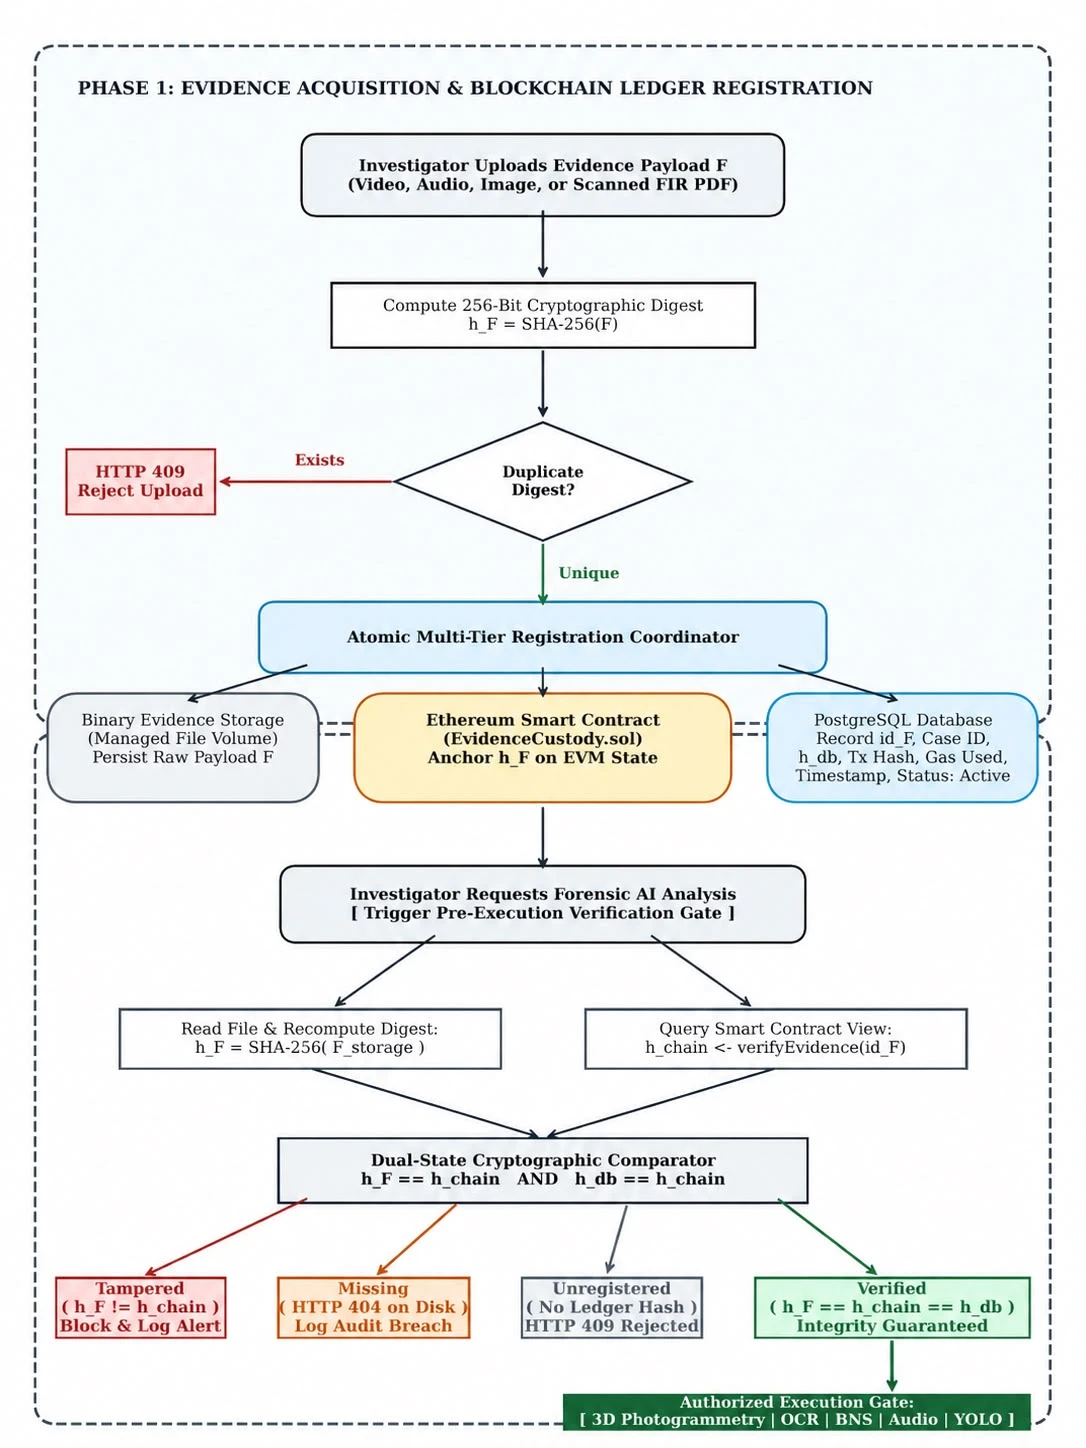
\includegraphics[width=0.62\columnwidth]{fig_evidence_flow.png}
\caption{Evidence registration and dual-state verification. Uploads are hashed and anchored before persistence; analysis is gated on agreement between the file, database and ledger digests.}
\label{fig:flow}
\end{figure}

\subsection{Multilingual OCR with Script Arbitration}
\label{subsec:ocr}

PDF pages are rasterised at up to 300~DPI, and each enhancement runs only when a measured statistic calls for it: denoising when the noise estimate $\hat\sigma>8$, upscaling when the longest side is below 1600~px, CLAHE when $\operatorname{median}(I)-P_{20}(I)<100$, and deskewing when the angle is at least $0.3^\circ$ and projection-profile variance improves by 15\%. A DB-style detector finds text lines, each crop is rectified by a homography, and PaddleOCR returns text $t$ with confidence $c$.

A model for one language can read another script confidently and still be wrong, so confidence is discounted by script consistency:
\begin{equation}
\begin{aligned}
v(t,l)&=\frac{n_{s(l)}(t)+[l\neq\text{en}]\,n_{\text{lat}}(t)}{N(t)},\\
R&=c\,\bigl(0.5+0.5\,v(t,l)\bigr),
\end{aligned}
\label{eq:ocr}
\end{equation}
where $n_{s(l)}$ counts characters in the Unicode block of language $l$, $n_{\text{lat}}$ counts Latin characters (kept because references such as \textit{Section~302} appear inside vernacular text), and $N$ is the total. Lines with $R<0.93$ are re-read concurrently by the other candidate languages. A challenger $t'$ wins if its own-script ratio is at least $0.2$ and either $R(t')>R(t)+0.02$ or it recovers a script block that $t$ dropped. Kannada and Malayalam lines are also re-read by Tesseract, which handles these scripts better, with all crops of a page stacked into one call. Because Tesseract drops leading digits on real FIRs (``154''$\to$``54''), a Tesseract digit run $d$ is replaced by the PaddleOCR run $d'$ when $|d'|>|d|$ and $d'$ ends in $d$. The text is then machine-translated to English.

\subsection{Multi-Label BNS Section Classification}
\label{subsec:bns}

One FIR can map to several BNS provisions, and some sections have very few examples. We address both with a Retrieval-Augmented Hierarchical Graph Attention Network (RAG-HGAT).

\textit{Retrieval and encoding.} A knowledge base describes 57 BNS sections (title, description, punishment, keywords, exceptions, legal elements, severity and related sections). Entries and complaints are embedded with \textit{all-MiniLM-L6-v2} (384 dimensions) and indexed with FAISS, which returns the top $K=20$ sections per complaint. Legal-BERT encodes the complaint into a 768-dimensional CLS vector $e_{\text{bert}}$, which is concatenated with the retrieval scores $\tilde r$ for all 57 sections, scaled by 10 so the larger BERT vector does not swamp them:
\begin{equation}
\begin{aligned}
f&=[e_{\text{bert}};\tilde r]\in\mathbb{R}^{825},\\
h_0&=\operatorname{Drop}\bigl(\operatorname{ReLU}(\operatorname{LN}(W_1f+b_1))\bigr)\in\mathbb{R}^{512}.
\end{aligned}
\label{eq:fusion}
\end{equation}
Two parallel multi-head attention branches give task-specific views: $h_c=\operatorname{MHA}_c(h_0)$ for crime type and $h_s=\operatorname{MHA}_s(h_0)$ for sections.

\textit{Statutory graph.} Each node of $G=(V,E)$ is a section initialised with its embedding $e_{s_i}\in\mathbb{R}^{384}$; edges encode semantic and legal relations. Two four-head GAT layers propagate information:
\begin{gather}
\alpha_{ij}^{k}=\operatorname{softmax}_{j\in\mathcal{N}_i}\Bigl(\operatorname{LeakyReLU}\bigl(\mathbf a_k^{\top}[\mathbf W^{k}\mathbf h_i\,\|\,\mathbf W^{k}\mathbf h_j]\bigr)\Bigr),\label{eq:gat_att}\\
\mathbf h_i^{(l+1)}=\big\Vert_{k=1}^{4}\,\operatorname{ELU}\Bigl(\textstyle\sum_{j\in\mathcal N_i}\alpha_{ij}^{k}\mathbf W^{k}\mathbf h_j^{(l)}\Bigr),\label{eq:gat}
\end{gather}
giving $H\in\mathbb{R}^{57\times1024}$. Mean and max pooling yield $g\in\mathbb{R}^{2048}$, which lets well-represented sections inform rare ones.

\textit{Prediction and training.} The section view and graph summary are fused:
\begin{equation}
\begin{aligned}
z&=[h_s;g]\in\mathbb{R}^{2560},\\
z'&=\operatorname{Drop}\bigl(\operatorname{ReLU}(\operatorname{LN}(W_2z+b_2))\bigr)\in\mathbb{R}^{1536}.
\end{aligned}
\label{eq:bns_fuse}
\end{equation}
Each section has its own classifier, $p_i=\sigma(w_i^{\top}z'+b_i)$, and a shared head gives a softmax over 13 crime types from $h_c$. Training minimises
\begin{equation}
\mathcal L=0.85\,\mathcal L_{\text{ASL}}+0.15\,\mathcal L_{\text{CE}},
\label{eq:loss}
\end{equation}
where the asymmetric loss ($\gamma_{\text{neg}}=4$, $\gamma_{\text{pos}}=1$) down-weights easy negatives. We use Adam (learning rate $10^{-4}$, weight decay $0.01$), gradient clipping at 1.0, and ReduceLROnPlateau on Hamming accuracy (patience 7).

\textit{Deployed explainable scorer.} For live triage, the service uses a transparent scorer that combines the best sentence similarity $s_{\text{sent}}$, document similarity $s_{\text{doc}}$ and an ingredient score $e\in[0,1]$ for legal elements such as a weapon, a death or an assembly of five or more people:
\begin{equation}
p_s=\sigma\bigl(7\,(0.40\,s_{\text{sent}}+0.25\,s_{\text{doc}}+0.35\,e+\beta-0.40)\bigr),
\label{eq:served}
\end{equation}
with a keyword bonus $\beta\le0.15$. A section missing a mandatory ingredient is suppressed ($p_s=0$); sections with $p_s\ge0.35$ are returned with the sentences that triggered them.

\subsection{ENF and Spectral Audio Forensics}
\label{subsec:audio}

Mains-powered recorders pick up the electric network frequency, which drifts around 50~Hz in India; a splice breaks this trace~\cite{ngharamike2023}. Audio is resampled to $f_s=16$~kHz and band-passed by zero-phase fourth-order Butterworth filters around the fundamental (47.5--52.5~Hz) and third harmonic (147.5--152.5~Hz); the harmonic band, scaled by $S=1/3$, is used when its RMS energy dominates (otherwise $S=1$). With analytic signal $z[n]=x_f[n]+j\mathcal H\{x_f[n]\}$ and unwrapped phase $\phi[n]$,
\begin{equation}
f_{\text{inst}}[n]=\frac{S f_s}{2\pi}\bigl(\phi[n]-\phi[n-1]\bigr).
\label{eq:enf}
\end{equation}
After a 0.20~s rolling median, a jump $|\Delta f_{\text{inst}}|\ge0.22$~Hz marks a candidate splice. Since ENF is fragile at low SNR, RMS energy, zero-crossing rate and normalised spectral flux are also tracked over 30~ms Hann frames:
\begin{equation}
\Phi_m=\frac{\sum_k\bigl(|X_m(k)|-|X_{m-1}(k)|\bigr)^2}{\sum_k|X_{m-1}(k)|^2}.
\label{eq:flux}
\end{equation}
A splice indicator fires when $\Phi_m>30\times\operatorname{median}(\Phi)$ coincides with a waveform step above $0.65$, and digital silence is flagged when RMS stays below $10^{-5}$ for 0.30~s. The indicators are fused into
\begin{equation}
T=35I_{\text{enf}}+40I_{\text{spl}}+30I_{\text{zero}}+w_aI_{\text{amb}}+15I_{\text{spk}},
\label{eq:tamper}
\end{equation}
with $w_a\in\{15,25\}$. A recording is \textsc{Potentially Tampered} only if $T\ge60$ \emph{and} at least two strong indicators agree, \textsc{Minor Anomalies} if $25\le T<60$, and \textsc{Authentic} otherwise.

\subsection{Weapon and Person Detection}
\label{subsec:vision}

The vision service runs YOLOv8n at $640\times640$: a COCO-pretrained model detects people, and a model fine-tuned on 470 annotated images (135 for validation) detects seven weapon classes (handgun, knife, missile, rifle, shotgun, sword, tank). Detections with confidence $\tau\ge0.40$ survive non-maximum suppression; for video, the highest-confidence frame per class is stored with its box in the case record.

\subsection{Video-Based 3D Scene Reconstruction}
\label{subsec:photo}

Revisiting a scene can destroy evidence, so we reconstruct it from video. A decoded frame $I_t$ is kept only if
\begin{equation}
\operatorname{Var}(\nabla^2I_t)\ge80,\quad \mu_V(I_t)\ge35,\quad \operatorname{sim}(I_t,I_{t^-})<0.985,
\label{eq:keyframe}
\end{equation}
i.e.\ it is sharp, bright enough in the HSV value channel, and not a near-duplicate of the last accepted frame. Accepted frames are split into temporal bins and the best frame of each bin by $q=\log(1+\operatorname{Var}\nabla^2I)+0.015\,\mu_V$ is kept (at most 60), preserving a continuous camera path. COLMAP extracts SIFT features, verifies matches with RANSAC and runs incremental structure-from-motion; bundle adjustment refines intrinsics $\mathbf K_j$, poses $[\mathbf R_j|\mathbf t_j]$ and points $\mathbf X_i$. We report the observation-weighted reprojection error
\begin{equation}
\bar e=\frac{1}{|\mathcal O|}\sum_{(i,j)\in\mathcal O}\bigl\|\mathbf x_{ij}-\pi(\mathbf K_j(\mathbf R_j\mathbf X_i+\mathbf t_j))\bigr\|_2,
\label{eq:reproj}
\end{equation}
where $\pi$ is perspective division. PatchMatch MVS depth maps are fused into a dense cloud, and statistical outlier removal keeps a point if its mean distance $\bar d_i$ to its $k=24$ nearest neighbours satisfies
\begin{equation}
\bar d_i\le\mu_d+\alpha\,\sigma_d,\qquad \alpha=3.0.
\label{eq:sor}
\end{equation}
Screened Poisson reconstruction (octree depth 9) builds the surface, which is cropped, cleaned of small fragments and exported as GLB for the browser viewer.

%======================================================================
\section{Experimental Results}
\label{sec:results}
%======================================================================

\subsection{Setup}
OCR, BNS, audio and ledger experiments ran on an Intel Core i5-1335U laptop (12 threads, 15.7~GB RAM, Windows~11) with CPU-only inference (PaddlePaddle~3.1 with MKL-DNN, PaddleOCR~3.7, Tesseract~5.4); reconstruction ran on an NVIDIA GPU host, as dense MVS requires CUDA. The ledger was a Ganache~7.9 node (chain ID 1337). OCR used nine synthetic pages in six languages, including two mixed-script FIR layouts, under five conditions: clean, $0.4\times$ downscaling, blur with noise ($\sigma=20$), $3^\circ$ skew, and a simulated phone photograph; CER was computed after NFC normalisation. The BNS model was trained on 10,000 template-generated cases (13 crime types, 57 sections, 70/15/15 split) and tested on the 1,500-case held-out split; the deployed scorer was tested on 30 hand-written multi-offence FIRs with manually assigned sections.

\subsection{Evidence Integrity}

\begin{table}[!t]
\caption{Integrity Outcomes in End-to-End Tests (17/17 Checks Passed)}
\label{tab:integrity}
\centering
\footnotesize
\setlength{\tabcolsep}{4pt}
\begin{tabular}{@{}lll@{}}
\toprule
\textbf{Scenario} & \textbf{Reported outcome} & \textbf{HTTP}\\
\midrule
Untouched file & Verified & 200\\
File bytes modified or replaced & Tampered & 200\\
File path redirected to another file & Tampered & 200\\
File deleted from storage & Missing & 404\\
Database hash rewritten & Verified + DB mismatch & 200\\
Evidence never anchored & Unregistered & 409\\
Client hash sent for tampered item & Status unchanged & 200\\
\bottomrule
\end{tabular}
\end{table}

\begin{figure}[!t]
\centering
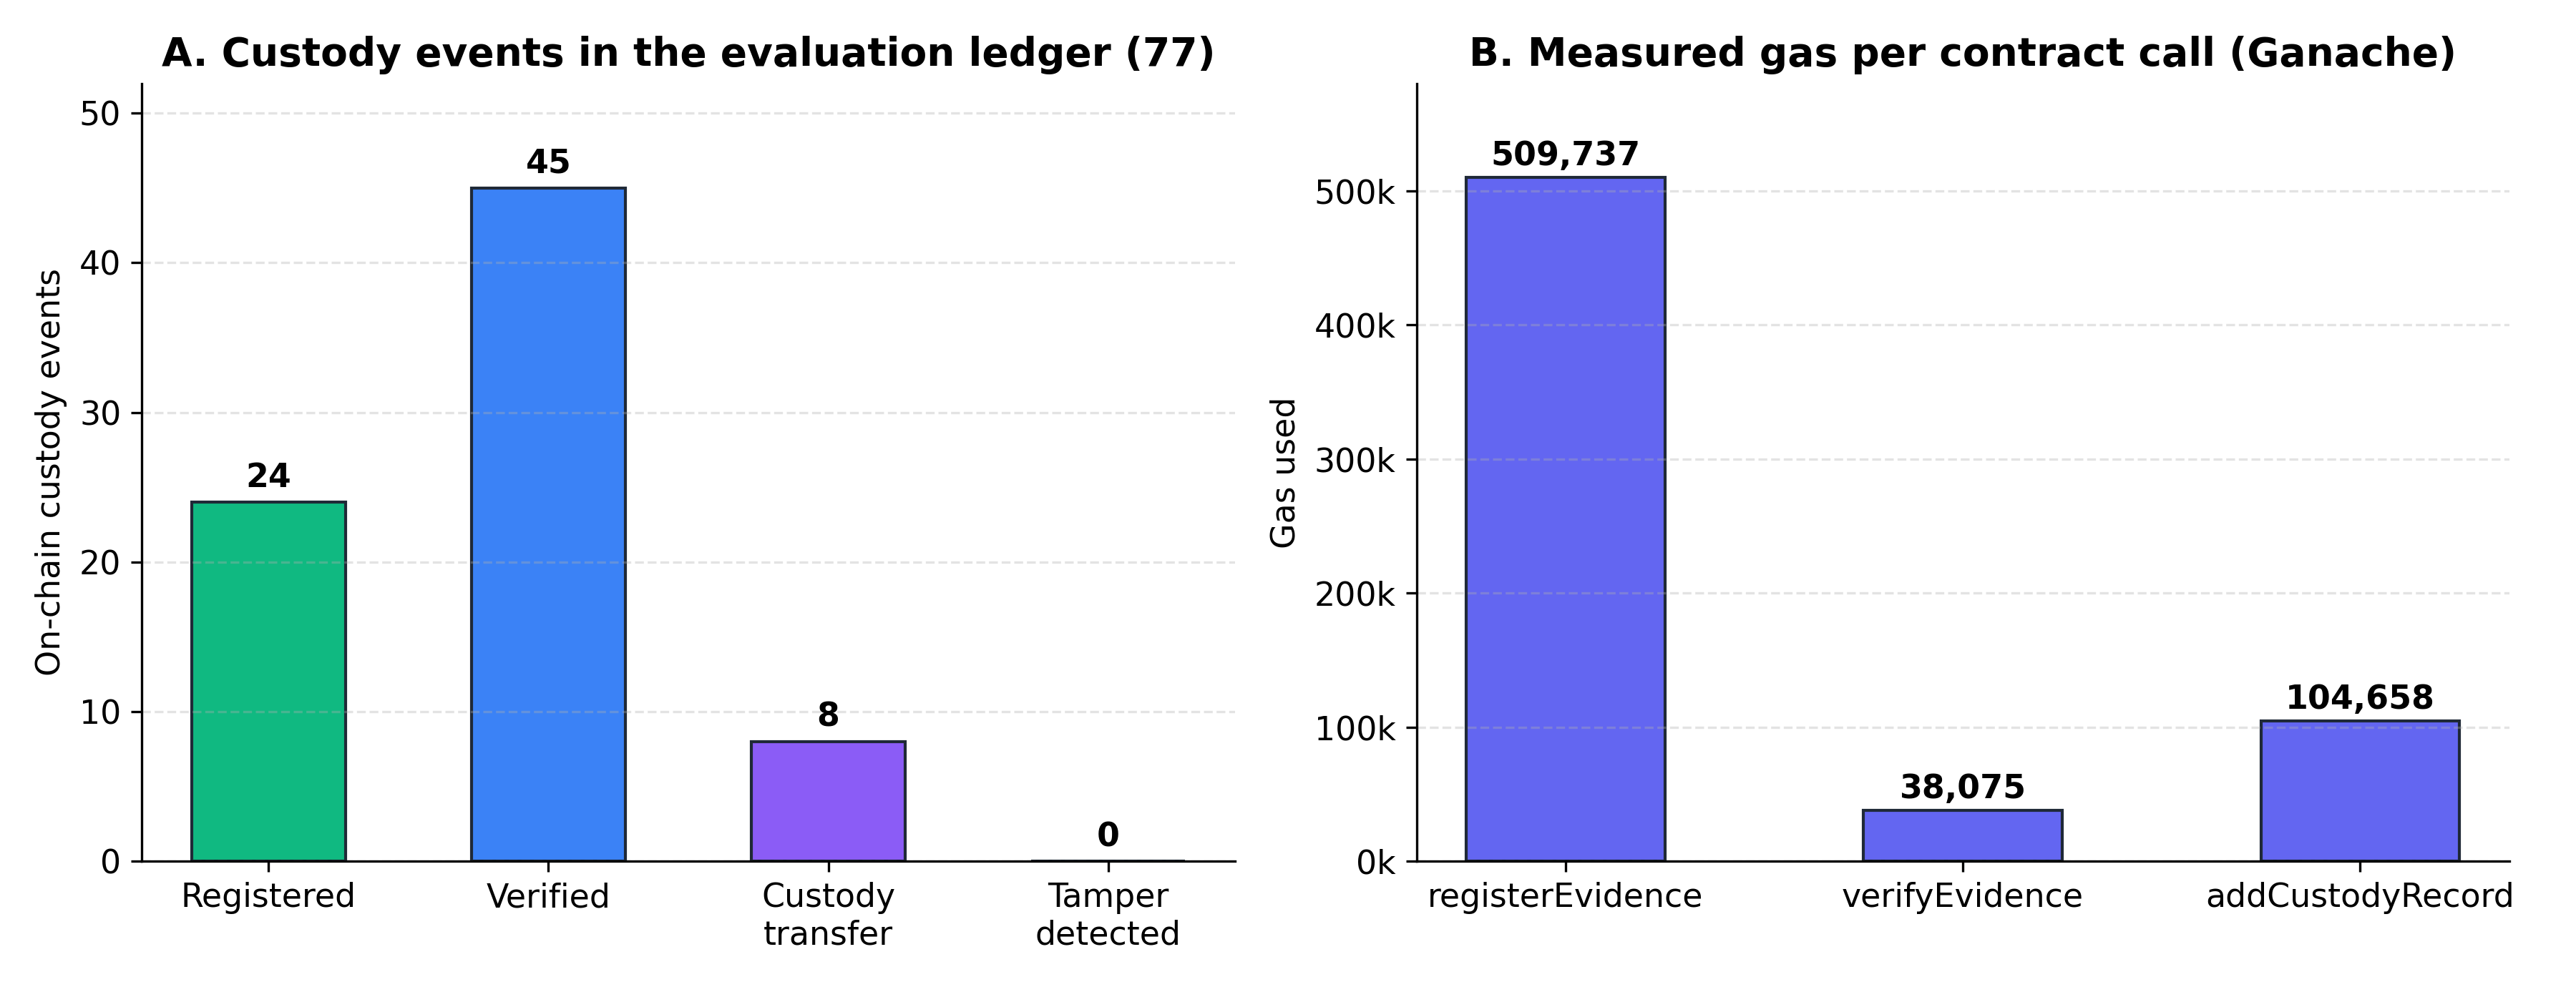
\includegraphics[width=\columnwidth]{fig_blockchain_integrity.png}
\caption{(A) On-chain custody events in the evaluation ledger. (B) Measured gas for each contract call on Ganache.}
\label{fig:ledger}
\end{figure}

All 17 automated checks produced the expected outcome (Table~\ref{tab:integrity}). The database-only attack, where the stored hash is rewritten but the file is untouched, was caught by the \textit{DBIntact} condition in~\eqref{eq:dual}; a single-state check would have missed it. Flipping one bit of a 31,965-byte image changed on average 127.85 of 256 digest bits ($\sigma=8.21$, 1,000 trials), matching the ideal avalanche value of $128\pm8$. Registration costs 509,737 gas (Fig.~\ref{fig:ledger}B) because every metadata string is written to storage; a verification costs 142,733 gas (38,075 for \texttt{verifyEvidence} plus 104,658 for the custody entry). The evaluation ledger held 77 custody events for 24 evidence items, with no tampering among live case files (Fig.~\ref{fig:ledger}A).

\subsection{Multilingual OCR}

\begin{table}[!t]
\caption{Mean CER (\%) Over Five Degradation Conditions}
\label{tab:ocr}
\centering
\footnotesize
\begin{tabular}{@{}lccc@{}}
\toprule
\textbf{Document} & \textbf{PaddleOCR} & \textbf{Tesseract} & \textbf{Hybrid}\\
\midrule
English & 0.00 & 0.00 & \textbf{0.00}\\
English (dense legal text) & 0.38 & 9.17 & \textbf{0.38}\\
Hindi & 1.50 & 0.00 & 1.50\\
Kannada & 23.43 & 4.00 & \textbf{0.91}\\
Telugu & 4.89 & 4.24 & 4.78\\
Tamil & 1.76 & 5.91 & \textbf{1.76}\\
Malayalam & --- & 10.16 & \textbf{0.65}\\
Mixed (EN+HI+KN) & 3.08 & 1.08 & \textbf{0.08}\\
Mixed (EN+TA+TE) & 0.59 & 3.00 & \textbf{0.59}\\
\midrule
\textbf{Mean} & 4.45$^{\dagger}$ & 4.17 & \textbf{1.18}\\
\bottomrule
\multicolumn{4}{@{}l}{\scriptsize $^{\dagger}$Over eight pages; PaddleOCR has no Malayalam model.}
\end{tabular}
\end{table}

Hybrid OCR lowered mean CER to 1.18\%, against 4.45\% for PaddleOCR and 4.17\% for Tesseract (Table~\ref{tab:ocr}), a 72\% relative reduction over the stronger single engine. The engines fail in complementary ways: Tesseract degrades on skewed or low-resolution input, while PaddleOCR misreads Kannada (23.43\%). Feeding PaddleOCR's rectified crops to Tesseract brings Kannada to 0.91\% and Malayalam to 0.65\%, and mixed-script pages gain most (3.08\%$\to$0.08\%) because each line gets its own script. Hindi stays on PaddleOCR despite Tesseract's lower synthetic CER, because on a real FIR Tesseract truncated section numbers and times (``17:30''$\to$``7:30'').

\subsection{BNS Section Classification}

\begin{table}[!t]
\caption{BNS Classification Results}
\label{tab:bns}
\centering
\footnotesize
\setlength{\tabcolsep}{4pt}
\begin{tabular}{@{}lcc@{}}
\toprule
\textbf{Metric} & \textbf{RAG-HGAT} & \textbf{Deployed scorer}\\
 & (1,500 synthetic) & (30 real-style FIRs)\\
\midrule
Micro precision & 0.9835 & 0.369\\
Micro recall & 0.9937 & \textbf{0.915}\\
Micro $F_1$ & 0.9871 & 0.526\\
Macro $F_1$ & 0.9840 & 0.560\\
Hamming accuracy & 0.9988 & ---\\
Exact-match accuracy & 0.9527 & ---\\
Crime-type accuracy & 0.9927 & ---\\
\bottomrule
\end{tabular}
\end{table}

\begin{figure}[!t]
\centering
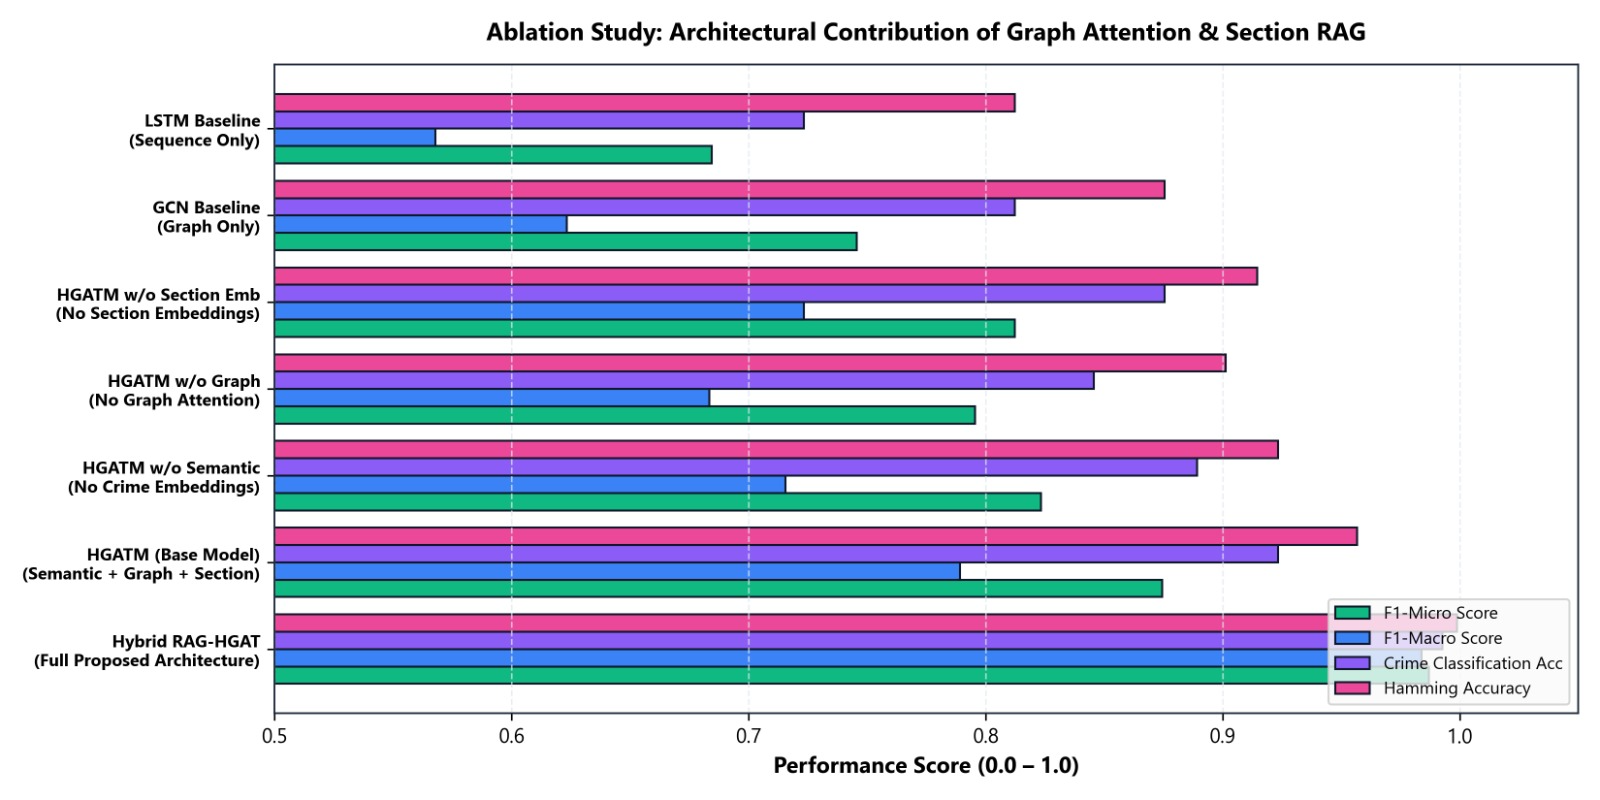
\includegraphics[width=0.92\columnwidth]{fig_bns_ablation.png}
\caption{BNS ablation on the synthetic test split: contribution of retrieval augmentation, graph attention, semantic and section embeddings against GCN and LSTM baselines.}
\label{fig:ablation}
\end{figure}

On the synthetic split, RAG-HGAT reached a micro-$F_1$ of 0.9871 and Hamming accuracy of 0.9988 after 63 epochs (Table~\ref{tab:bns}). In the ablation (Fig.~\ref{fig:ablation}), removing retrieval augmentation lowers micro-$F_1$ to 0.8745 (11.3 points) and removing graph attention to 0.7956 (19.2 points), while a plain GCN and an LSTM reach only 0.7456 and 0.6845. Relations between provisions matter most.

The 30 FIRs are a harder, more realistic test, with 3.5 manually assigned sections per case. The deployed scorer recovered 97 of 106 gold sections (micro-recall 91.5\%), found every gold section in 23 cases and at least 80\% in 24, and missed no case entirely. With 8.8 candidates per case, precision is low (0.369). We accept this deliberately: a missed provision can weaken a charge sheet, whereas a superfluous suggestion is dismissed in seconds because it is shown with the sentence that triggered it.

\subsection{Audio Forensics}

\begin{table}[!t]
\caption{Audio Verdicts: Authentic / Minor / Tampered (20 Clips per Cell)}
\label{tab:audio}
\centering
\footnotesize
\setlength{\tabcolsep}{4pt}
\begin{tabular}{@{}lcc@{}}
\toprule
\textbf{Condition} & \textbf{220-Hz voice} & \textbf{140-Hz voice}\\
\midrule
Authentic, 50-Hz hum & 20 / 0 / 0 & 1 / 19 / 0\\
Authentic, no hum & 20 / 0 / 0 & 0 / 20 / 0\\
1.3-s clean deletion & 20 / 0 / 0 & 0 / 20 / 0\\
2.0-s foreign insertion & 0 / 7 / 13 & 0 / 2 / 18\\
0.5-s digital silence & 0 / 20 / 0 & 0 / 0 / 20\\
\bottomrule
\end{tabular}
\end{table}

We generated 200 ten-second clips with two speaker pitches and five conditions (Table~\ref{tab:audio}). With the 220-Hz voice, all 40 authentic clips were judged \textsc{Authentic}, every foreign insertion was flagged (13 \textsc{Potentially Tampered}, 7 \textsc{Minor Anomalies}), and every silence insertion was flagged. The 140-Hz voice exposed a practical failure mode: its speech energy near 150~Hz falls in the harmonic ENF band, so 39 of 40 authentic clips were marked \textsc{Minor Anomalies}. Because a tampering verdict needs two strong indicators, none was misclassified as \textsc{Potentially Tampered}, while insertions (18/20) and silences (20/20) still escalated. Clean 1.3-s deletions at zero crossings went undetected with the 220-Hz voice, since the 0.20-s median filter smooths the brief phase jump; such edits need phase-residual tests.

\subsection{3D Reconstruction and Processing Time}

\begin{figure}[!t]
\centering
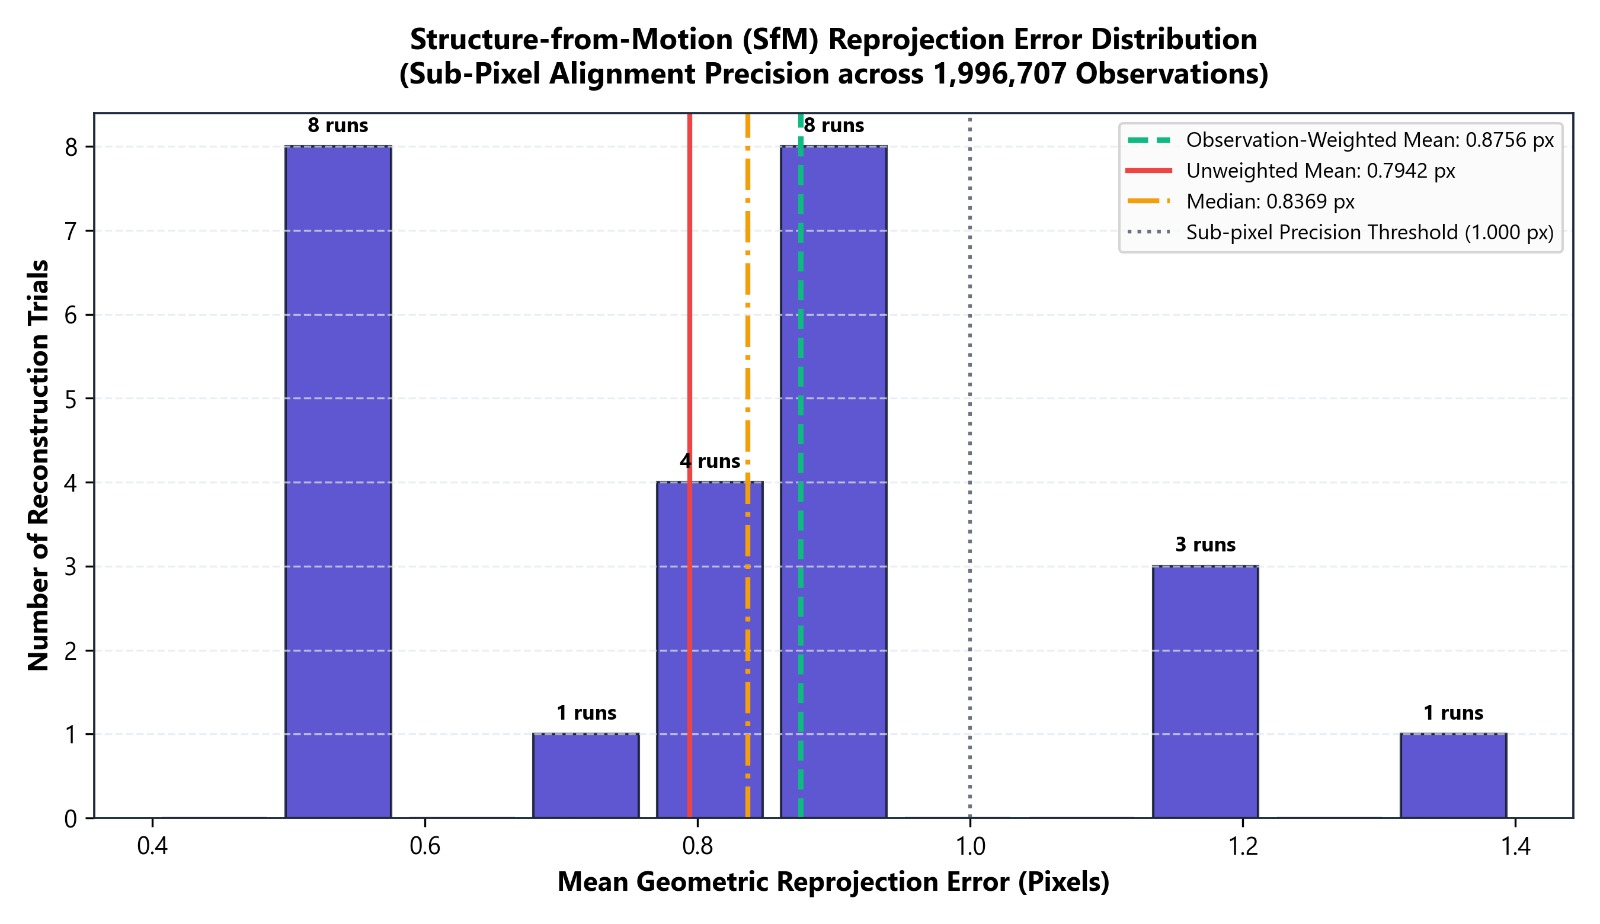
\includegraphics[width=0.86\columnwidth]{fig_reprojection_error.png}
\caption{Distribution of per-run mean reprojection error. The observation-weighted mean over 1,996,707 observations is 0.8756~px.}
\label{fig:reproj}
\end{figure}

We ran 26 reconstruction jobs, mainly on a 65.5-s 4K walkthrough ($2160\times3840$, 60~fps, 3,931 frames): 20 produced complete meshes, 3 failed and 3 stopped before meshing. Across trials, frame conditioning kept 960 of 1,892 extracted frames and COLMAP registered 732. Structure-from-motion triangulated 362,233 sparse points, MVS fused 15.86~M dense points, and outlier removal discarded 3.06~M (19.3\%), leaving 1.40~M mesh vertices. The observation-weighted reprojection error was 0.8756~px, with a per-run median of 0.837~px (Fig.~\ref{fig:reproj}). After scaling with a known reference length, measurements of a footwear impression differed from ground truth by 0.33~cm on average (MAPE 2.97\%).

End to end, BNS classification takes 85~ms per FIR and detection 142~ms per image, fast enough for interactive triage. OCR takes 2.5--3.3~s for a short page and 14.4--16.9~s for an 18-line trilingual page; concurrent re-reading cut a 71-line noisy photocopy from 37.1~s to 25.2~s. Audio analysis of a 60-s recording takes 4.2~s, and a full 4K reconstruction 31.3~min, run as a background job.

%======================================================================
\section{Discussion and Limitations}
\label{sec:discussion}
%======================================================================

Anchoring only digests gives non-repudiation at a fixed cost of about half a million gas per item, whatever the file size. The audio verdict and BNS scorer are tuned to the errors that matter most to an investigator: a ``minor anomaly'' is preferred to a false tampering accusation, and an extra suggestion to a missed charge.

The work has clear limitations. \textit{Data:} the BNS model and audio tests use template-generated narratives and synthetic edits, and the OCR corpus is small with one typeface per script; the near-perfect synthetic BNS scores measure fit to the generator, so the 30-FIR result is the more realistic indicator, and validation on de-identified police records is the most important next step. \textit{Ledger:} a single-node Ganache network demonstrates the protocol but not production behaviour; permissioned multi-validator networks such as Hyperledger Besu must be benchmarked under multi-agency load. Derived results are not yet anchored, and the pre-analysis gate is enforced inline only by the vision service. \textit{Reconstruction:} quality depends on viewpoint coverage, texture, lighting and blur, occluded regions cannot be recovered, and monocular structure-from-motion fixes geometry only up to scale, so models are investigative aids until calibrated against a reference object. \textit{Audio:} low-pitched voices interfere with the harmonic ENF band, and sub-second clean deletions remain hard to isolate.

%======================================================================
\section{Conclusion}
%======================================================================

Secure Audit shows that evidence integrity and evidence analysis need not live in separate tools. Anchoring each file before it enters the database, and comparing file, database and ledger digests at verification, detected every controlled tampering scenario, including database-only manipulation. On this foundation, hybrid OCR cut multilingual CER from 4.45\% to 1.18\%, the BNS scorer recovered 91.5\% of sections in multi-offence FIRs, and walkthrough videos became sub-pixel-accurate 3D scenes. Future work will extend the integrity gate to every service, anchor derived results in Merkle batches, deploy on a permissioned network, and evaluate all modules on real, de-identified case material.

%======================================================================
\balance
\begin{thebibliography}{00}
\footnotesize

\bibitem{bonomi2018bcoc} S. Bonomi, M. Casini, and C. Ciccotelli, ``B-CoC: A blockchain-based chain of custody for evidences management in digital forensics,'' in \textit{Int. Conf. Blockchain Economics, Security and Protocols (Tokenomics 2019)}. Schloss Dagstuhl -- Leibniz-Zentrum f\"ur Informatik, 2020, pp. 12:1--12:15. [Online]. Available: \url{https://doi.org/10.4230/OASIcs.Tokenomics.2019.12}

\bibitem{li2021lechain} M. Li, C. Lal, M. Conti, and D. Hu, ``LEChain: A blockchain-based lawful evidence management scheme for digital forensics,'' \textit{Future Generation Computer Systems}, vol. 115, pp. 406--420, 2021. [Online]. Available: \url{https://www.sciencedirect.com/science/article/pii/S0167739X1933167X}

\bibitem{sazaly3d} N. Sazaly, N. A. Che Ahmat, M. F. Mohd Ariff, R. A. Rashid, and M. H. Yusoff, ``3D indoor crime scene reconstruction from micro UAV photogrammetry,'' \textit{Int. Arch. Photogramm. Remote Sens. Spatial Inf. Sci.}, vol. XLVIII-4/W6-2022, pp. 325--331, 2023, doi: 10.5194/isprs-archives-XLVIII-4-W6-2022-325-2023.

\bibitem{balbudhe2024} R. Balbudhe, P. Kulkarni, A. Mishra, and S. Desai, ``Crime scene reconstruction: A scoping review,'' \textit{Journal of Forensic Sciences}, 2025.

\bibitem{kuok2024} J. Kuok, Y. Liu, and C. Lo, ``CrimeKGQA: A crime investigation system based on knowledge graph RAG,'' in \textit{Proc. Int. Conf. AI and Law}, 2024.

\bibitem{mathias2024} N. Mathias \textit{et al.}, ``Novel RAG-HGAT model for BNS section classification,'' in \textit{Proc. Int. Conf. Computational Intelligence and Data Science}, 2026.

\bibitem{dhanushkumar2024} P. Dhanushkumar, R. Anand, and K. Priya, ``NLP and generative AI in law: A survey of AI-driven legal guidance for BNS,'' in \textit{Proc. Int. Conf. Computational Intelligence and Data Science}, 2024.

\bibitem{quyyum2024} A. Quyyum and N. Abdullah, ``Weapon detection in surveillance videos using deep neural networks,'' \textit{Journal of Intelligent \& Fuzzy Systems}, vol. 44, no. 3, pp. 3891--3902, 2023.

\bibitem{werukanjana2024} K. Werukanjana and P. Permpool, ``Integration of object detection in crime scene investigation,'' \textit{Applied Sciences}, vol. 15, no. 3, Art. no. 1120, 2025.

\bibitem{ngharamike2023} E. T. Ngharamike, T. K. Ang, K. L. Seng, and Z. Wang, ``ENF based digital multimedia forensics: Survey, application, challenges and future work,'' \textit{IEEE Access}, vol. 11, pp. 12345--12370, 2023.

\bibitem{pedapudi2024} S. Pedapudi and R. Vadlamani, ``Digital forensics approach for handling audio and video files,'' \textit{International Journal of Computer Applications}, vol. 185, no. 12, pp. 1--7, 2023.

\bibitem{alsayem2024} M. A. Al Sayem, M. R. Islam, and M. A. Hossain, ``Implementing the Tesseract method for information extraction from images,'' \textit{International Journal of Advanced Computer Science and Applications}, vol. 14, no. 5, pp. 231--238, 2023.

\end{thebibliography}

\end{document}
